\section{Kinematics and Timing of Signal and Background events}
\label{sec:kinematics_and_timing}

\subsection{0\nbb-decay signal and 2\nbb-decay background}

In both 0\nbb-decay signal and 2\nbb-decay background events near the decay energy spectrum endpoint, the kinematics of the
electron pair is very similar. Large fraction of events have a nearly back-to-back topology with a close to 
equal energy split between electrons. To simulate 0\nbb- and 2\nbb-decay events we use a Monte Carlo generator based on phase 
factors from Ref.~\cite{Jenni}. Similarity in kinematics of 0\nbb- and 2\nbb-decay events is demonstrated in Fig.~\ref{fig:Kinematics}.

The electron angular correlations for 0\nbb-decay are noticeably different from 2\nbb-decay due to a contribution from the
neutrino wave-functions even at vanishingly small energies of the neutrinos~\cite{Jenni}. However, any practical use of this difference 
in separating 0\nbb-decay from 2\nbb-decay would require extremely large number of candidate events. Given the half-time of 2\nbb-decay 
and upper limits on the half-time of 0\nbb-decay, electron angular correlations will not bring a decisive separation power in controlling 
2\nbb-decay background in currently planned 0\nbb-decay experiments. Excellent energy resolution at the Q-value remains the key parameter
in 2\nbb~background suppression.

While we do not exclude that the angular correlations as an input to a multivariative technique may improve sensitivity of 0\nbb-decay 
searches, in this paper we assume that there is no difference in the event topology between 0\nbb-~and 2\nbb-decay events. Any conclusions 
about 0\nbb-decay events also hold for 2\nbb-decay when the total energy of the electrons in 2\nbb-decay events is close to the Q-value.


\begin{figure*}[ht]
  \centering
  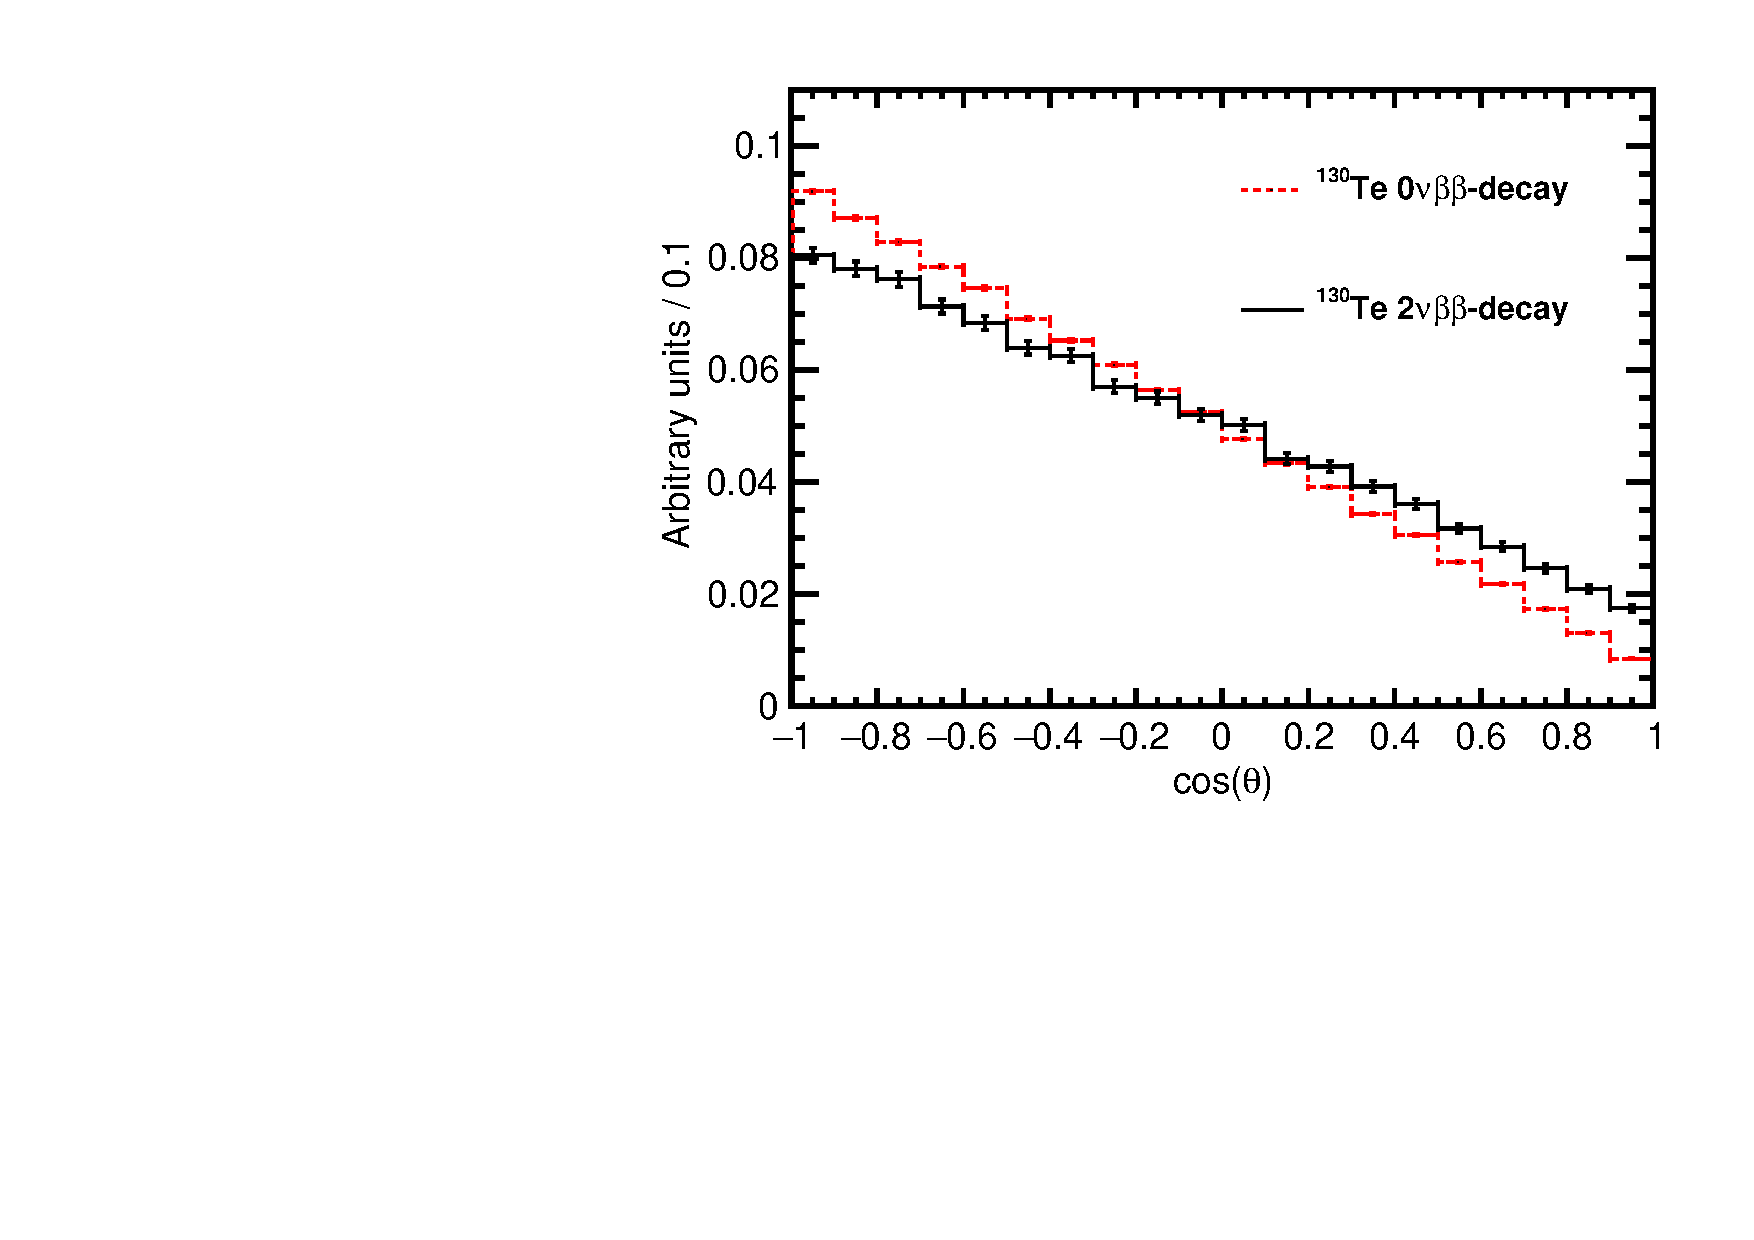
\includegraphics[width=0.49\textwidth]{hCos_Te130.pdf}
  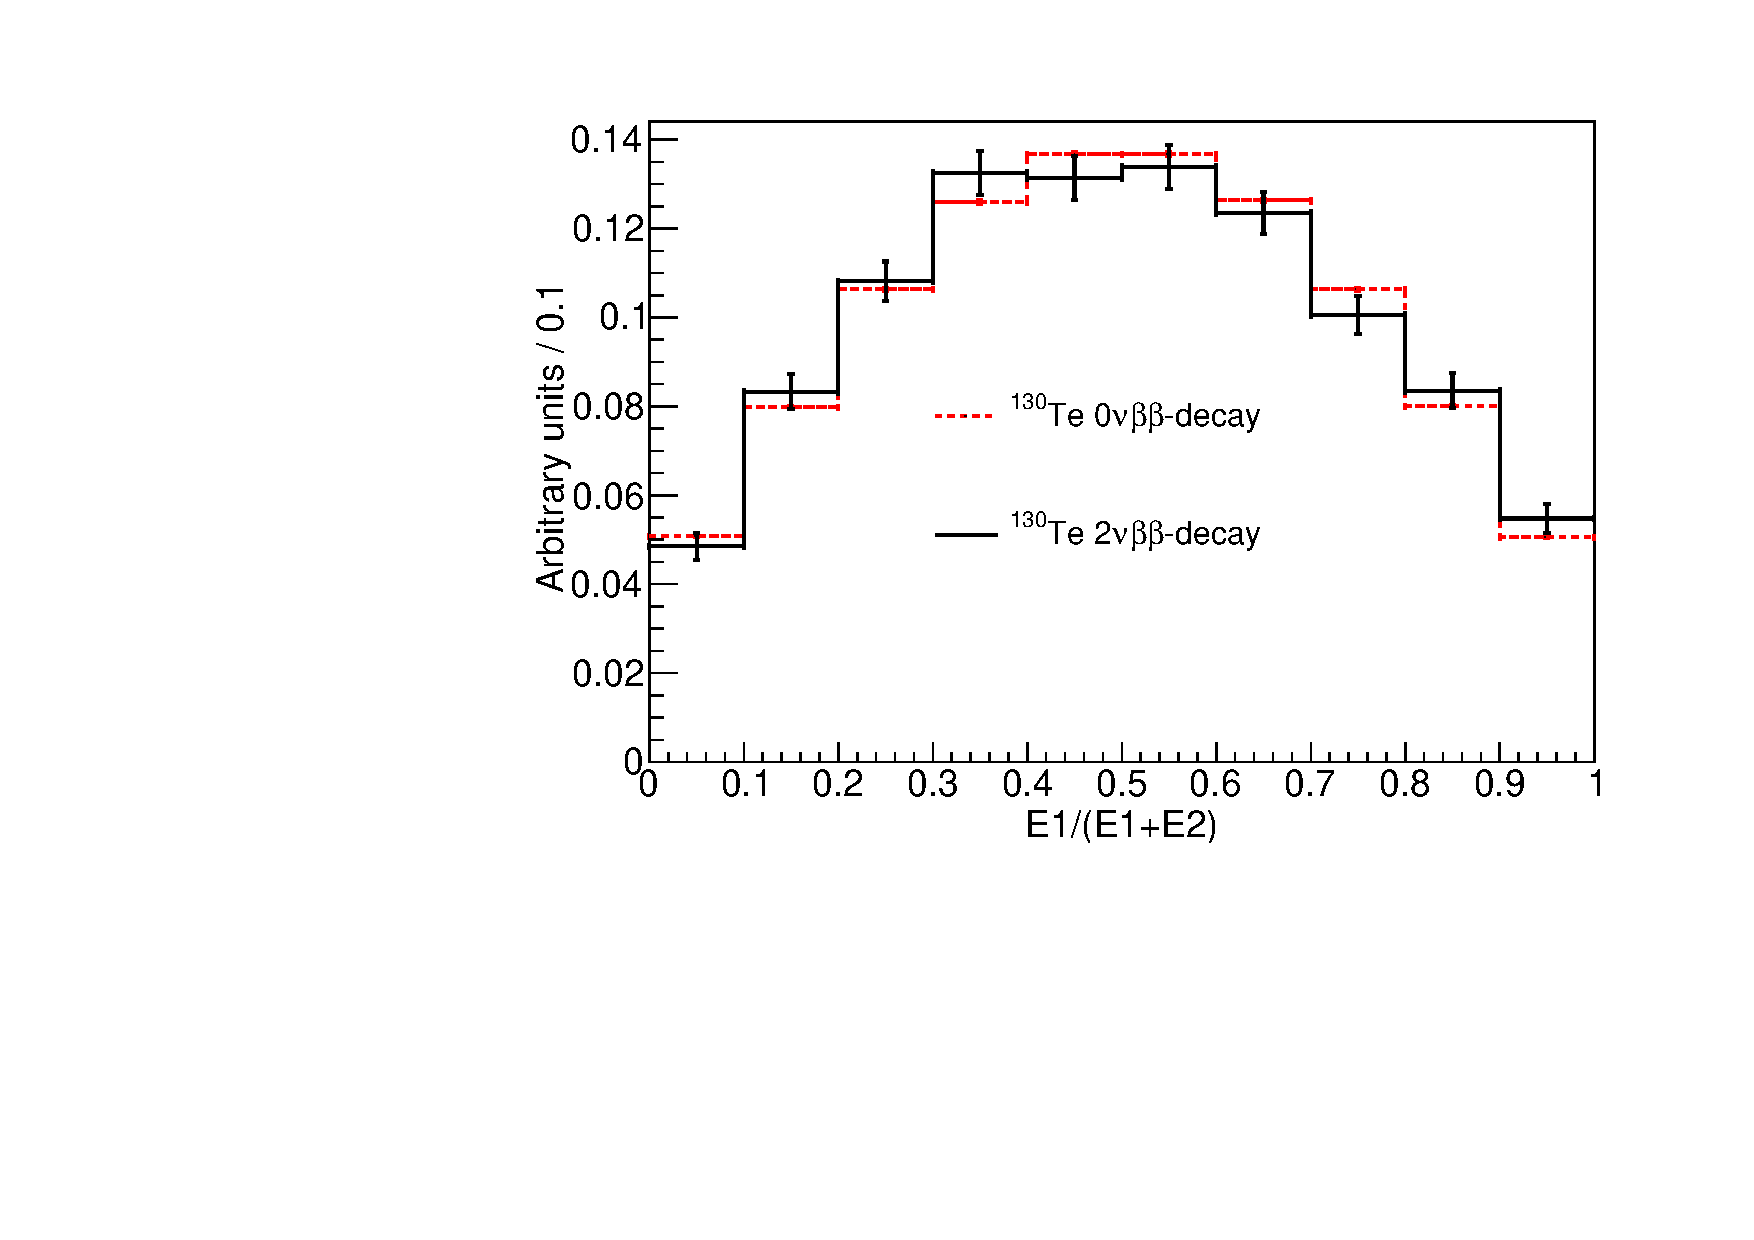
\includegraphics[width=0.49\textwidth]{hE1toQ_Te130.pdf}
  \caption{Comparison between kinematics of 0{\nbb} (\emph{dashed red
      lines}) and 2{\nbb} decays (\emph{solid black lines}) for events
    with the total kinetic energy of the electrons above 90\% of the
    Q-value. \emph{Left:} Cosine of the angle between two
    electrons. \emph{Right:} Fraction of energy carried by one of the
    two electrons. Vertical bars at each bin of the histograms indicate
    statistical uncertainty for that bin.}
  \label{fig:Kinematics}
\end{figure*}


%Should we recalculate for 130Te.
Examining the kinematics for one of the 0\nbb~electrons with equal energy split, a 1.26~MeV electron travels a total path length of 0.X~cm, 
has a distance from the origin of 0.X~cm in 0.0X$\pm$0.00X~ns  and takes 0.0X$\pm$0.00X~ns to drop below Cherenkov threshold. 
We note that due to scattering of the electron, the final direction of the electron before it stops does not correspond to the initial 
direction; however the scattering angle is small at the time the majority of Cherenkov light is produced.

Figure~\ref{fig:ArrivalTimeDist} shows the output of the detector simulation for 1000 simulated \Te~ 0\nbb-decay 
events. The left-hand panel in Fig.~\ref{fig:ArrivalTimeDist} compares PE arrival time between Cherenkov and scintillation light.
The right-hand panel shows the composition of the early PE sample, which is key to direction and topographical reconstruction, 
selected with the time cut of 33.5~ns. Each \Te~ 0\nbb-decay produces total of 6X$\pm$X PEs in the early PE sample. 
There are 3X$\pm$X scintillation and 3X$\pm$X Cherenkov PEs.


\begin{figure*}[ht]
  \centering
  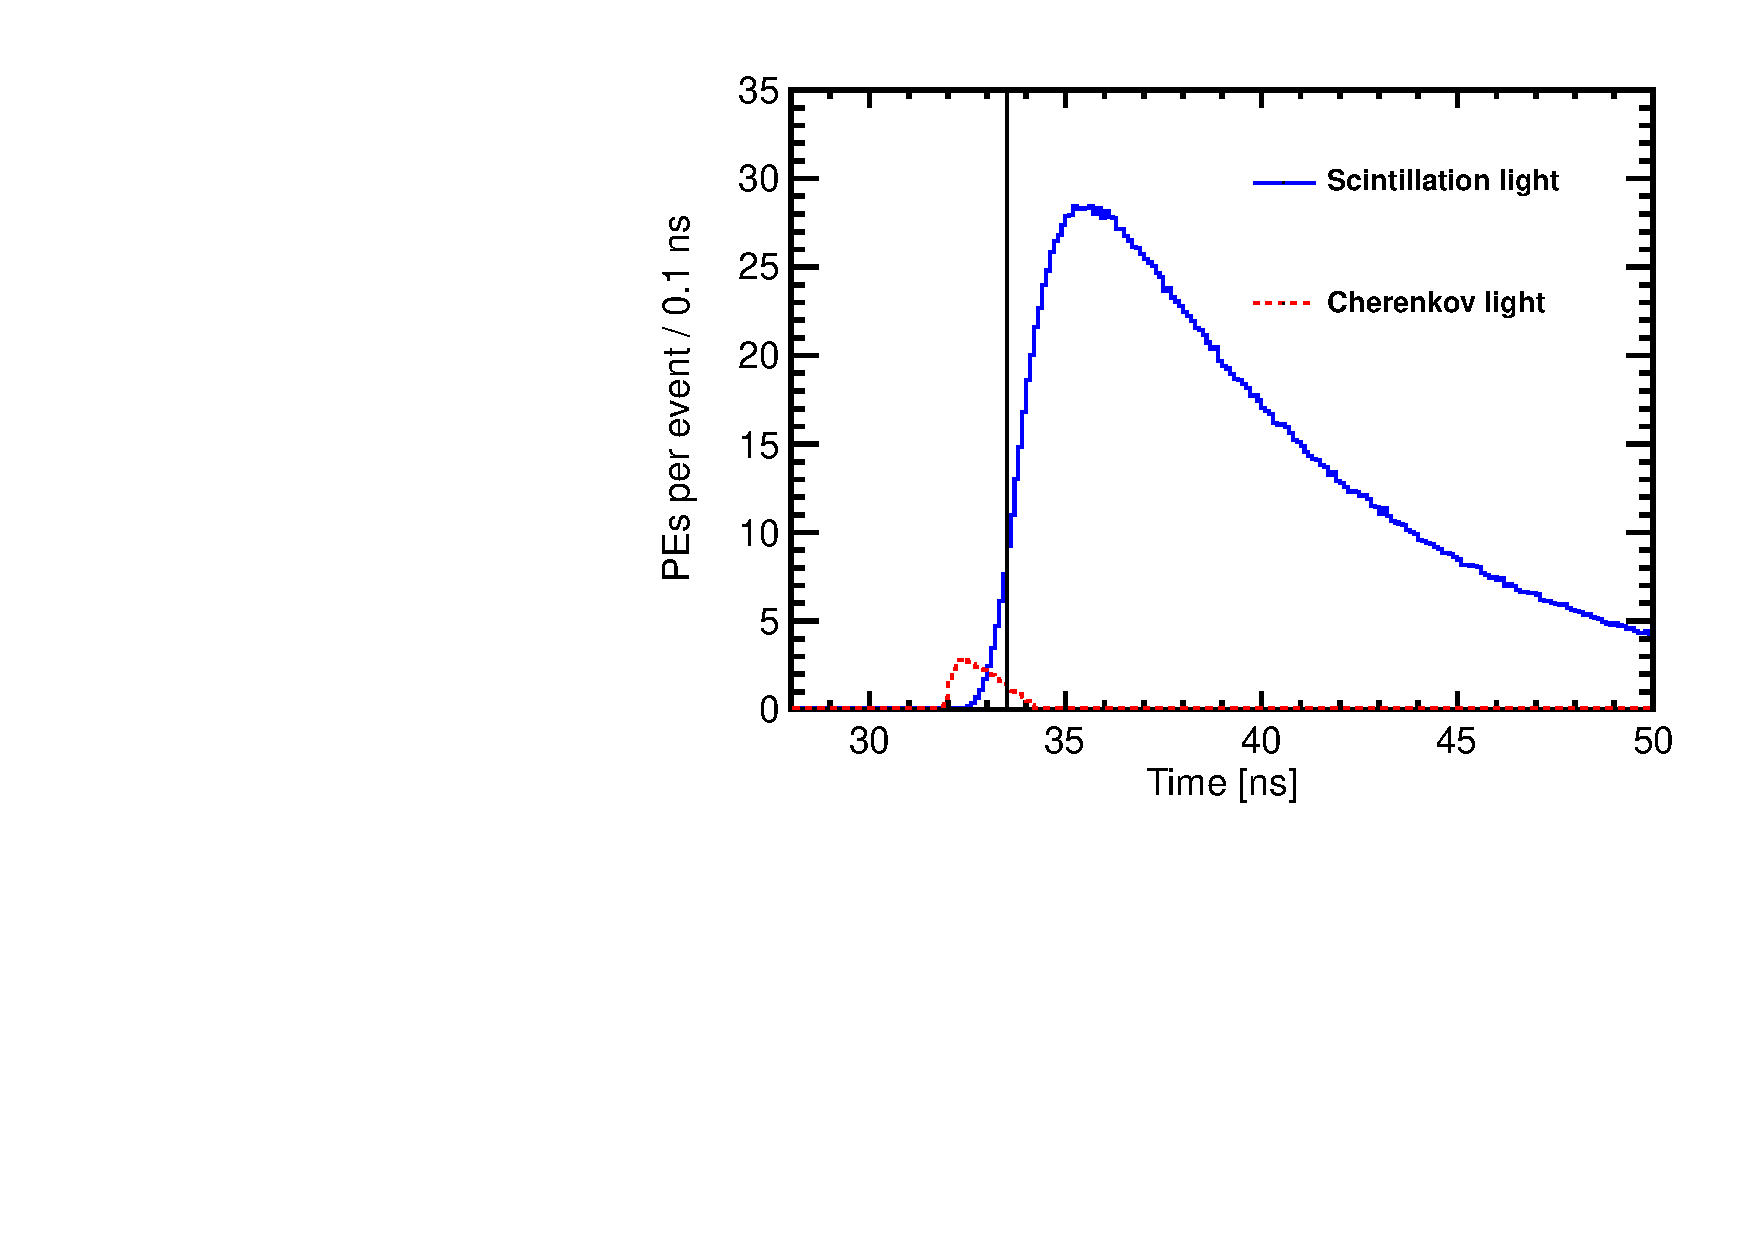
\includegraphics[width=0.45\textwidth]{hT_Te130.pdf}
  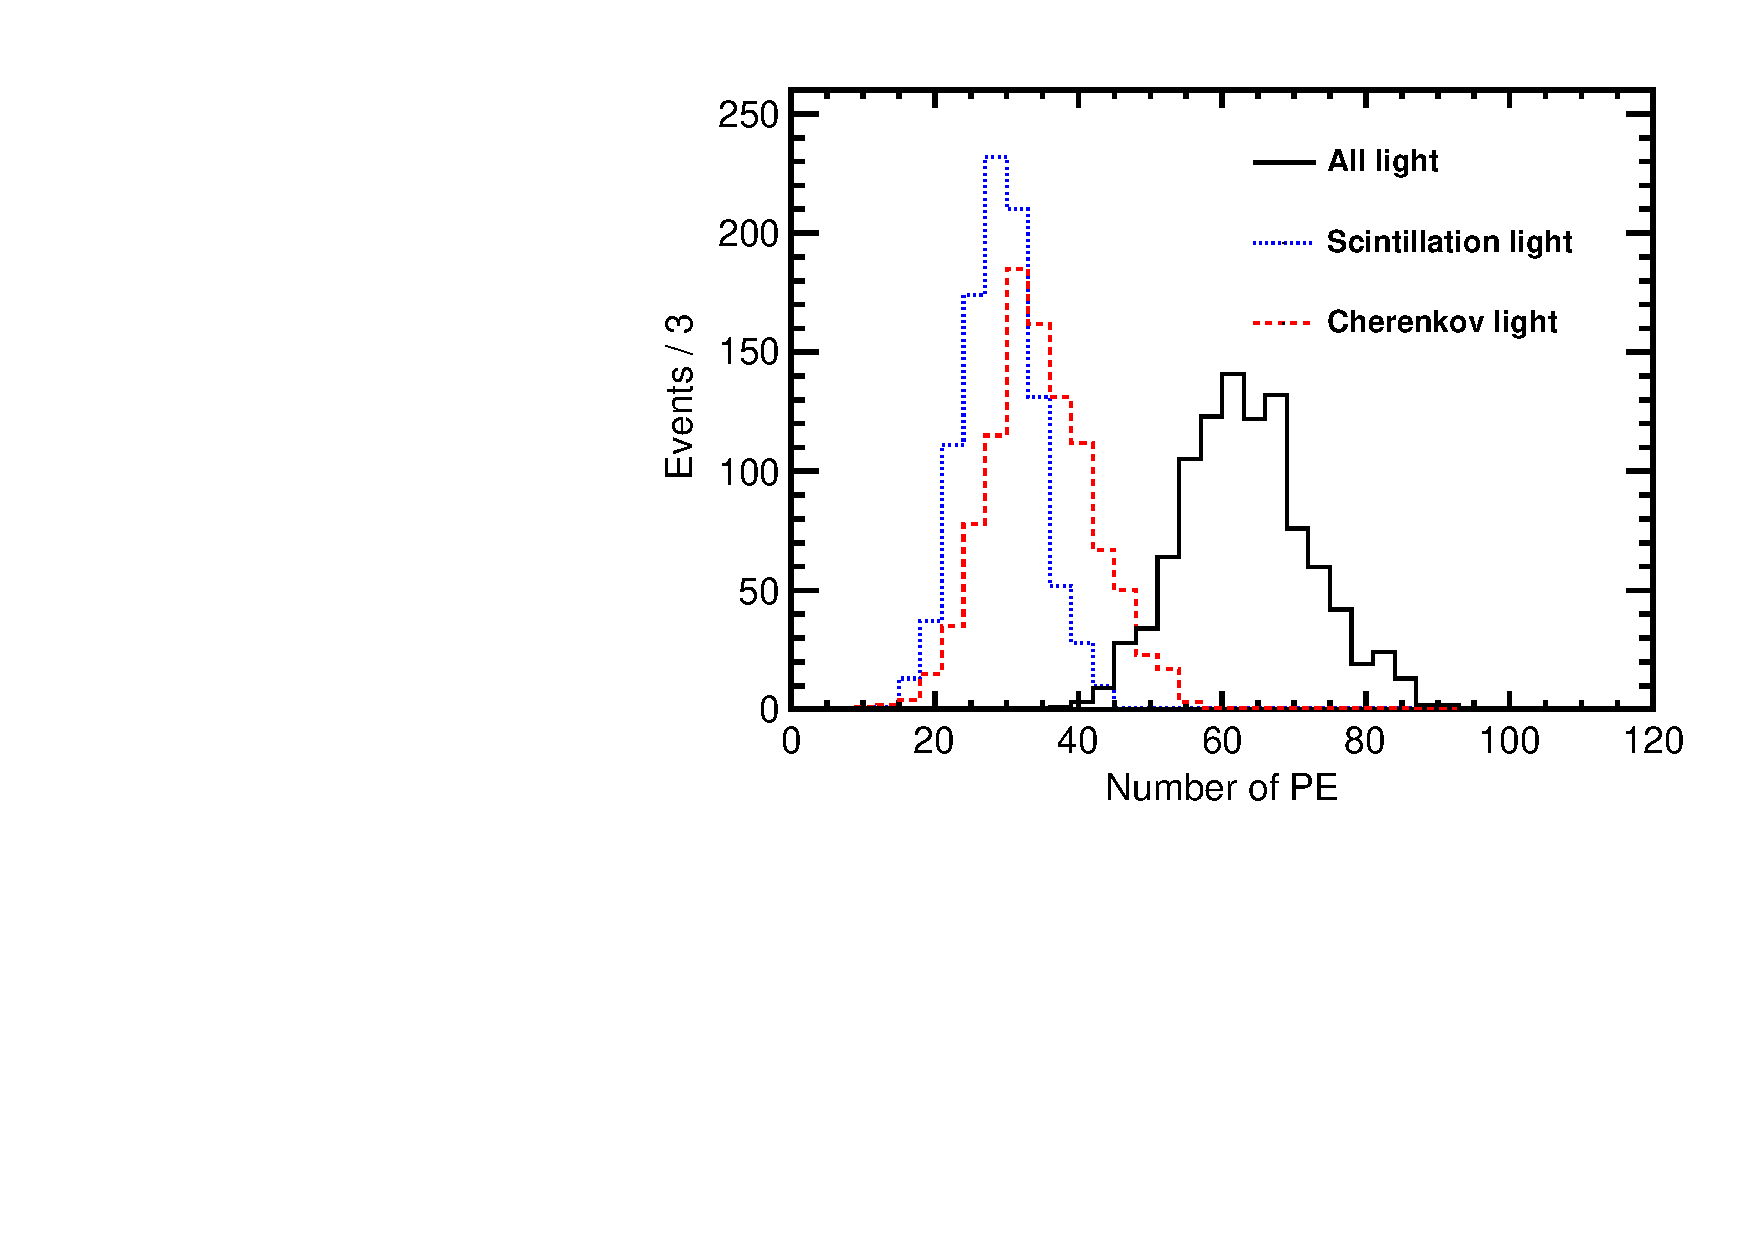
\includegraphics[width=0.45\textwidth]{hMomNPhot_Te130.pdf}
  \caption{\emph{Left:} Photo-electron (PE) arrival times after
    application of the photo-detector transit time spread (TTS) of 100~ps for the default simulation 
    of \Te~0\nbb-decay produced at the center of the detector. 
    Scintillation PEs (blue solid line) are compared to Cherenkov PEs (red dotted line)
    The vertical line at 33.5~ns indicates the time cut for the selection of the early PE sample.
    \emph{Right:} Composition of the early PE sample: 
    number of Cherenkov (\emph{dashed red line}), scintillation (\emph{dotted blue line}), 
    and total (\emph{solid black line}) PEs per event.} 
\label{fig:ArrivalTimeDist}
\end{figure*}


Selection of PEs with relatively small arrival time allows the selection of a sample of PEs with a high fraction of directional Cherenkov light.
This allows for event topology reconstruction. In particular, signal-like events with exactly two electrons can be separated from events 
with only one electron such as from \B~solar neutrino interactions.


\subsection{\B~background}

For a detector similar to our model, \B~background is significant due to large total mass of the liquid scintillator in
the active region of the detector.
Electrons from elastic scattering of \B~solar neutrinos have nearly a flat energy spectrum around the 
Q-value~\cite{SNOp-B8-bkg}. We simulate \B~background as a single monochromatic electron with energy of 2.53~MeV 
(Q-value of \Te). A 2.53~MeV electron travels a total path length of 0.X~cm, has a distance from the origin of 0.X~cm in 
0.0X$\pm$0.00X~ns  and takes 0.0X$\pm$0.00X~ns to drop below Cherenkov threshold.

The shape of scintillation and Cherenkov PE timing distributions in \B~events match very closely the shape of corresponding distributions
for 0\nbb-decay events shown in Fig.~\ref{fig:ArrivalTimeDist}. The electron path length is too short compared to the detector size to 
introduce any noticable difference in the shape of PE timing distributions between a single electron from \B~events and two 
electrons from 0\nbb-events.

Each \B~event produces total of 7X$\pm$X PEs in the early PE sample. There are 3X$\pm$X scintillation and 4X$\pm$X Cherenkov PEs.
The total energy depositited in the detector in \B~and 0\nbb-decay events is the same. This leads to the same amount of 
scintillation light produced in the detector. The number of Cherenkov photons is slightly higher for \B~events because the Cherenkov 
light is being produced by a single electron with the same kinetic energy as the sum of kinetic energy of two electrons 
in 0\nbb-decay events. 

We do note use small difference in the total number of PEs in the early PE sample to separate 0\nbb-decay signal from \B~background.
However, it may provide an extra handle on signal-background separation in a multivariative analysis when combined with directional
and topographical information.

